\documentclass[tikz]{standalone}

\usepackage{xstring}

\usetikzlibrary{fit,positioning}

\begin{document}
    
    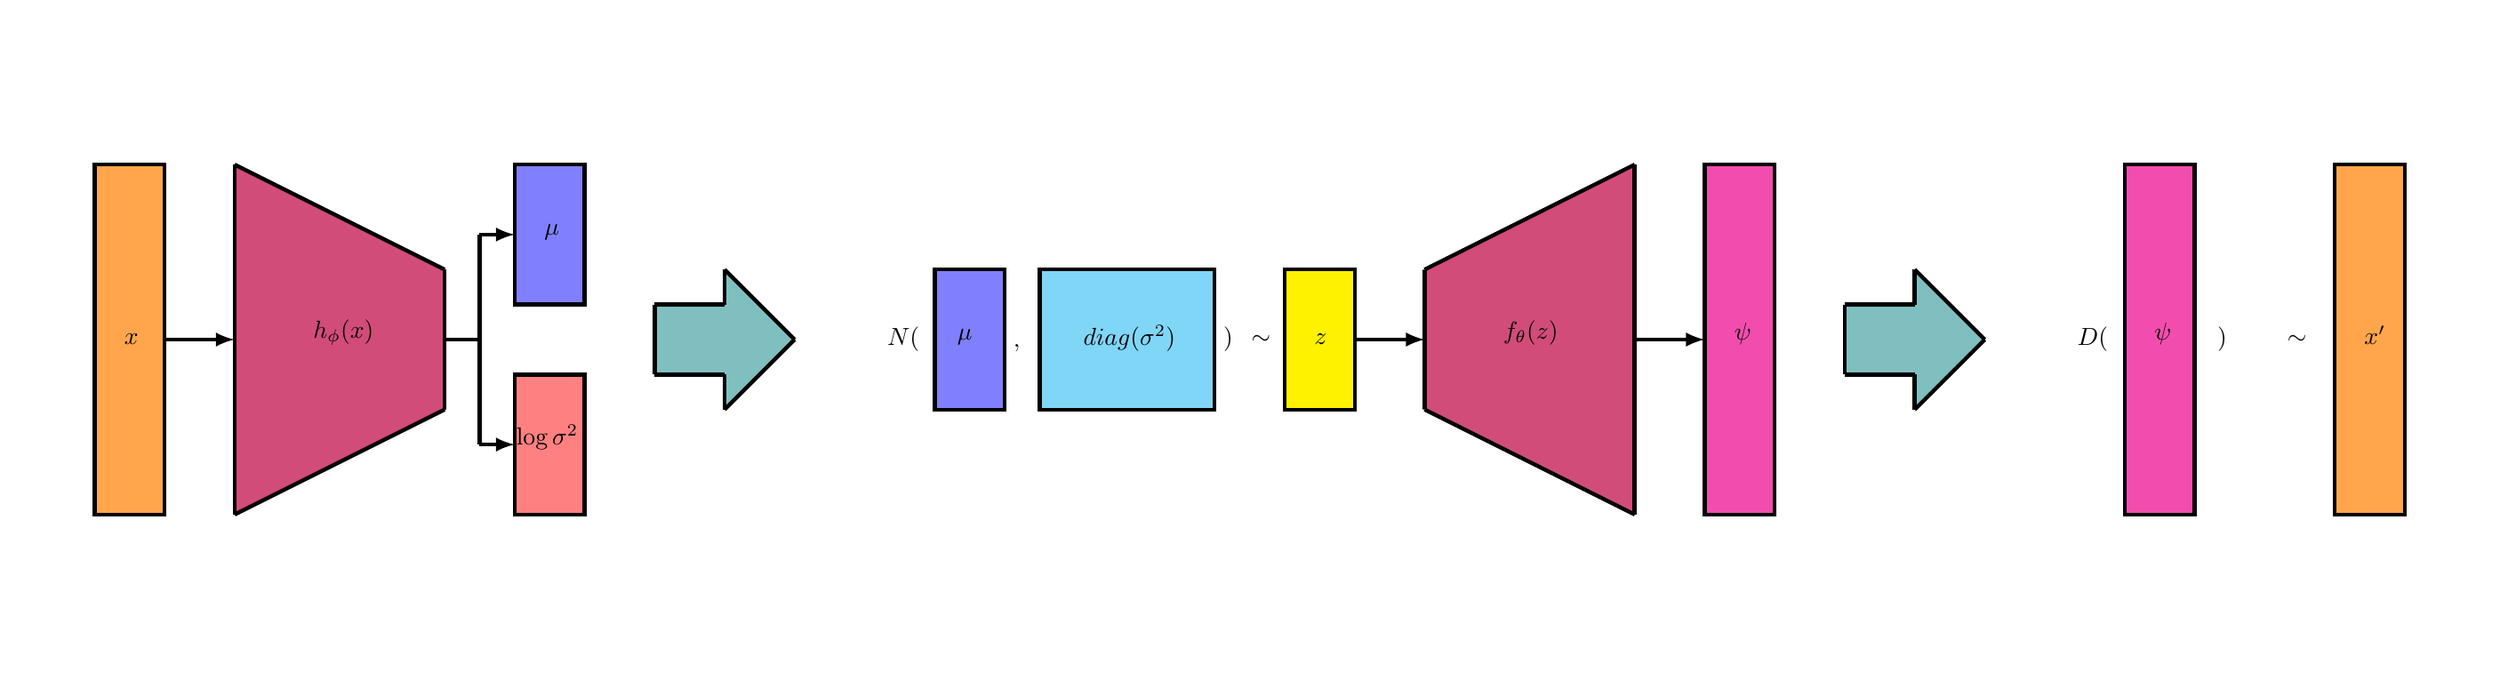
\begin{tikzpicture}
        \useasboundingbox (-16, 2) rectangle (19, -7);
        
	\draw[draw=black, ultra thick, solid, fill = orange!70] (-15.00,0.00) rectangle (-14.00,-5.00);
    
	\draw[draw=black, -latex, ultra thick, solid] (-14.00,-2.50) -- (-13.00,-2.50);

        \fill[purple!70] 
        (-13.00,0.00) -- 
        (-13.00,-5.00) -- 
        (-10.00,-3.50) -- 
        (-10.00,-1.50) -- 
        cycle;
        
	\draw[draw=black, ultra thick, solid] (-13.00,0.00) -- (-13.00,-5.00);
	\draw[draw=black, ultra thick, solid] (-13.00,-5.00) -- (-10.00,-3.50);
	\draw[draw=black, ultra thick, solid] (-13.00,0.00) -- (-10.00,-1.50);
	\draw[draw=black, ultra thick, solid] (-10.00,-1.50) -- (-10.00,-3.50);
	
        \draw[draw=black, ultra thick, solid] (-10.00,-2.50) -- (-9.50,-2.50);
    
	\draw[draw=black, ultra thick, solid, fill = blue!50] (-9.00,0.00) rectangle (-8.00,-2.00);
    
	\draw[draw=black, ultra thick, solid, fill = red!50] (-9.00,-3.00) rectangle (-8.00,-5.00);
    
	\draw[draw=black, ultra thick, solid] (-9.50,-2.50) -- (-9.50,-1.50);
	\draw[draw=black, ultra thick, solid] (-9.50,-1.50) -- (-9.50,-1.00);
	\draw[draw=black, ultra thick, solid] (-9.50,-2.50) -- (-9.50,-4.00);
    
	\draw[draw=black, -latex, ultra thick, solid] (-9.50,-1.00) -- (-9.00,-1.00);
    
	\draw[draw=black, -latex, ultra thick, solid] (-9.50,-4.00) -- (-9.00,-4.00);

        \fill[teal!50] 
        (-7.00,-2.00) -- 
        (-7.00,-3.00) -- 
        (-6.00,-3.00) -- 
        (-6.00,-3.50) -- 
        (-5.00,-2.50) -- 
        (-6.00,-1.50) -- 
        (-6.00,-2.00) -- 
        cycle;
        
	\draw[draw=black, ultra thick, solid] (-7.00,-2.00) -- (-7.00,-3.00);
	\draw[draw=black, ultra thick, solid] (-7.00,-2.00) -- (-6.00,-2.00);
	\draw[draw=black, ultra thick, solid] (-7.00,-3.00) -- (-6.00,-3.00);
	\draw[draw=black, ultra thick, solid] (-6.00,-2.00) -- (-6.00,-1.50);
	\draw[draw=black, ultra thick, solid] (-6.00,-1.50) -- (-5.00,-2.50);
	\draw[draw=black, ultra thick, solid] (-6.00,-3.00) -- (-6.00,-3.50);
	\draw[draw=black, ultra thick, solid] (-6.00,-3.50) -- (-5.00,-2.50);
    
	\draw[draw=black, ultra thick, solid, fill = blue!50] (-3.00,-1.50) rectangle (-2.00,-3.50);
    
	\draw[draw=black, ultra thick, solid, fill = cyan!50] (-1.50,-1.50) rectangle (1.00,-3.50);
    
	\draw[draw=black, ultra thick, solid, fill = yellow] (2.00,-1.50) rectangle (3.00,-3.50);

        \fill[purple!70] 
        (4.00,-1.50) -- 
        (7.00,0.00) -- 
        (7.00,-5.00) -- 
        (4.00,-3.50) -- 
        cycle;
        
	\draw[draw=black, ultra thick, solid] (4.00,-1.50) rectangle (4.00,-3.50);
	\draw[draw=black, ultra thick, solid] (4.00,-1.50) -- (7.00,0.00);
	\draw[draw=black, ultra thick, solid] (4.00,-3.50) -- (7.00,-5.00);
	\draw[draw=black, ultra thick, solid] (7.00,0.00) -- (7.00,-5.00);
    
	\draw[draw=black, ultra thick, solid, fill = magenta!70] (8.00,0.00) rectangle (9.00,-5.00);
    
	\draw[draw=black, -latex, ultra thick, solid] (3.00,-2.50) -- (4.00,-2.50);
	\draw[draw=black, -latex, ultra thick, solid] (7.00,-2.50) -- (8.00,-2.50);

        \fill[teal!50] 
        (10.00,-2.00) -- 
        (10.00,-3.00) -- 
        (11.00,-3.00) -- 
        (11.00,-3.50) -- 
        (12.00,-2.50) -- 
        (11.00,-1.50) -- 
        (11.00,-2.00) -- 
        cycle;
        
	\draw[draw=black, ultra thick, solid] (10.00,-2.00) -- (10.00,-3.00);
	\draw[draw=black, ultra thick, solid] (10.00,-2.00) -- (11.00,-2.00);
	\draw[draw=black, ultra thick, solid] (10.00,-3.00) -- (11.00,-3.00);
	\draw[draw=black, ultra thick, solid] (11.00,-3.00) -- (11.00,-3.50);
	\draw[draw=black, ultra thick, solid] (11.00,-2.00) -- (11.00,-1.50);
	\draw[draw=black, ultra thick, solid] (11.00,-3.50) -- (12.00,-2.50);
	\draw[draw=black, ultra thick, solid] (12.00,-2.50) -- (11.00,-1.50);

        \draw[draw=black, ultra thick, solid,  fill = magenta!70] (14.00,0.00) rectangle (15.00,-5.00);
	\draw[draw=black, ultra thick, solid,  fill = orange!70] (17.00,0.00) rectangle (18.00,-5.00);

	\node[black, anchor=south west] at (-14.7,-2.7) {$x$};
    
        \node[black, anchor=south west] at (-12,-2.7) {$h_\phi(x)$};

        \node[black, anchor=south west] at (-8.7,-1.2) {$\mu$};

        \node[black, anchor=south west] at (-9.1,-4.2) {$\log \sigma^2$};

        \node[black, anchor=south west] at (-3.8,-2.8) {$\Large N($};

        \node[black, anchor=south west] at (-2.8,-2.7) {$\mu$};

        \node[black, anchor=south west] at (-2,-2.8) {$\large ,$};

        \node[black, anchor=south west] at (-1,-2.8) {$diag(\sigma^2)$};

        \node[black, anchor=south west] at (1,-2.8) {$\large )$};

        \node[black, anchor=south west] at (1.4,-2.7) {$\large \sim$};

	\node[black, anchor=south west] at (2.3,-2.7) {$z$};
    
	\node[black, anchor=south west] at (5,-2.7) {$f_\theta(z)$};

        \node[black, anchor=south west] at (8.3,-2.7) {$ \psi $};

        \node[black, anchor=south west] at (13.2,-2.8) {$ D ( $};

        \node[black, anchor=south west] at (14.3,-2.7) {$ \psi $};

        \node[black, anchor=south west] at (15.2,-2.8) {$\large )$};
        
        \node[black, anchor=south west] at (16.2,-2.7) {$\large \sim$};

	\node[black, anchor=south west] at (17.3,-2.7) {$x'$};   
    
\end{tikzpicture}
\end{document}